\immediate\write18{makeindex phd_main.nlo -s nomencl.ist -o phd_main.nls}

\documentclass[a4paper,10pt]{report}


\usepackage[utf8]{inputenc}
\usepackage[T1]{fontenc}
\usepackage{amsmath}
\usepackage{amssymb}
\usepackage{array}
\usepackage{bibentry}
\usepackage{caption}
\usepackage{commath}
\usepackage{enumitem}
\usepackage{esint}
\usepackage{graphicx}
\usepackage{hyperref}
\usepackage{ifthen}
\usepackage{lipsum}
\usepackage{setspace}
\usepackage{subcaption}
\usepackage{tcolorbox}
\tcbuselibrary{breakable}
\usepackage{tikz}
\usepackage{xcolor}
\usepackage{siunitx}
% \usepackage[numbers]{natbib} % default citation with numbers
\usepackage[authoryear,round]{natbib} % http://merkel.texture.rocks/Latex/natbib.php
\usepackage[section]{placeins}
\setcounter{secnumdepth}{4}
\setcounter{tocdepth}{4}

\usepackage{fullpage} % reduces the margins of the template
\usepackage{afterpage}

%--------------------------------------------
% traits, tirets, pointillés
\usepackage{tikz}
\DeclareRobustCommand\full     {\tikz[baseline=-0.6ex]\draw[thick] (0,0)--(0.5,0);}
\DeclareRobustCommand\fullfat  {\tikz[baseline=-0.6ex]\draw[line width=2pt] (0,0)--(0.5,0);}
\DeclareRobustCommand\dotted   {\tikz[baseline=-0.6ex]\draw[thick,dotted] (0,0)--(0.54,0);}
\DeclareRobustCommand\dottedfat{\tikz[baseline=-0.6ex]\draw[line width=2pt,dotted] (0,0)--(0.54,0);}
\DeclareRobustCommand\dashed   {\tikz[baseline=-0.6ex]\draw[thick,dashed] (0,0)--(0.54,0);}
\DeclareRobustCommand\chain    {\tikz[baseline=-0.6ex]\draw[thick,dash dot dot] (0,0)--(0.5,0);}
% from: https://tex.stackexchange.com/questions/365707/legend-in-caption-dotted-chain-dashed-lines-in-pdflatex#365725
% --------------------------------------------


\usepackage{geometry}
\geometry{top=80pt, bottom=75pt, left=70pt, right=70pt}


%%%% Entetes et pieds de pages
\usepackage{fancyhdr}
\pagestyle{fancy}
\setlength{\headsep}{10pt} % https://tex.stackexchange.com/questions/136478/decrease-space-between-paragraph-and-header
\renewcommand{\chaptermark}[1]{\markboth{\chaptername~\thechapter{} : #1}{}}
\renewcommand{\sectionmark}[1]{\markright{\thesection{} \ #1}}
\renewcommand{\headrulewidth}{0.2pt}	
\renewcommand{\footrulewidth}{0.2pt}% Line at the footer visible
\fancyhf{}
\fancyhead[R]{\ifthenelse{\isodd{\value{page}}}{\textsl{\rightmark}}{}}
\fancyhead[L]{\ifthenelse{\isodd{\value{page}}}{}{\textsl{\leftmark}}}
\fancyfoot[R]{\ifthenelse{\isodd{\value{page}}}{\thepage}{}}
\fancyfoot[L]{\ifthenelse{\isodd{\value{page}}}{}{\thepage}}

%% Pieds de page pour les pages de chapitre
\fancypagestyle{plain}{
  \fancyhf{}
  \fancyfoot[R]{\ifthenelse{\isodd{\value{page}}}{\thepage}{}}
  \fancyfoot[L]{\ifthenelse{\isodd{\value{page}}}{}{\thepage}}
  \renewcommand{\headrulewidth}{0pt}% Line at the header invisible
  \renewcommand{\footrulewidth}{0.2pt}% Line at the footer visible
}



\AtBeginEnvironment{thebibliography}{\linespread{1}\selectfont}

\usepackage{nomencl}
\renewcommand\nomgroup[1]{%
  \ifthenelse{\equal{#1}{A}}{\item[\textbf{Acronyms}]}{% A - Acronyms
  \ifthenelse{\equal{#1}{R}}{\item[\textbf{Latin characters}]}{% R - Roman
  \ifthenelse{\equal{#1}{G}}{\item[\textbf{Greek characters}]}{% G - Greek
  \ifthenelse{\equal{#1}{S}}{\item[\textbf{Superscripts}]}{% S - Superscripts
  \ifthenelse{\equal{#1}{U}}{\item[\textbf{Subscripts}]}{% U - Subscripts
  \ifthenelse{\equal{#1}{X}}{\item[\textbf{Other}]}{% X - Other Symbols
  }}}}}}}
\renewcommand*{\nompreamble}{\markboth{\nomname}{\nomname}}
\newcommand{\nomunit}[1]{\renewcommand{\nomentryend}{\hspace*{\fill}#1}}
\makenomenclature

% Annexes
\usepackage[toc]{appendix}



\headheight=10pt

\setcounter{secnumdepth}{4}
\setcounter{tocdepth}{4}

%%%%%%%%%%.. def. chapitre %%%%%%%%%%%%%%%
\makeatletter
\def\@makechapterhead#1{%
  \vspace*{50\p@}%
  {\parindent \z@ \raggedright
   \interlinepenalty\@M
   \ifnum \c@secnumdepth >\m@ne
     \huge \bfseries \thechapter \quad
   \fi
   \huge \bfseries #1\par\nobreak
   \rule{\textwidth}{1mm}
   \vskip 40\p@
  }}

\def\@makeschapterhead#1{%
  \vspace*{50\p@}%
  {\parindent \z@ \raggedright
   \normalfont
   \interlinepenalty\@M
   \huge \bfseries #1\par\nobreak
    \vskip 40\p@
  }}
\makeatother
%%%%%%%%%%%%%%%%%%%%%%%%%%%%%%%%%%%%%%%%%%

%\input{macros}

\newcommand\blankpage{%
    \null
    \thispagestyle{empty}%
    %\addtocounter{page}{-1}%
    \newpage}
    
\newcommand\skippage{%
    \null
    %\thispagestyle{empty}%
    %\addtocounter{page}{-1}%
    \newpage}


%%% \renewcommand\partname{} %  so to remove the french occurences "première partie" % https://openclassrooms.com/forum/sujet/latex-modifier-le-texte-des-parties-chapitres-etc-10498

% to force chapter numbering to restart at each part:
\makeatletter
\@addtoreset{chapter}{part}
\makeatother

\parindent=0cm % "ds préambule, et plus besoin de \noindent !"
\graphicspath{{Images/}}




\begin{document}
\setlength{\unitlength}{1cm}



% Page de garde
% Pieds de page pour les pages de chapitre
\thispagestyle{empty}

\setstretch{1}

\begin{center}

\includegraphics[width=0.99\linewidth]{logo_UDL.eps}
\end{center}
N$^\circ$ d'ordre NNT: 1966LYSEC??
\vskip 2cm
\begin{center}
\textbf{\Large{TH\`ESE de DOCTORAT DE L'UNIVERSIT\'E DE LYON}}\\
\textbf{\Large{opérée au sein de l'\'Ecole Centrale de Lyon \\[3ex]
\'Ecole Doctorale N$^\circ$ 162}} \\
\textbf{\large{Mécanique \'Energétique Génie Civil Acoustique\\[3ex]
Spécialité de doctorat : Acoustique}} \\[5ex]
{\large{Soutenue publiquement le 16/12/1966, par \\[1ex]
\textbf{Monsieur Spock} }}
\end{center}

\vskip 8ex

\noindent
\rule{\textwidth}{1pt}

\begin{center}
{\LARGE{}
\textbf{Scientific Essay on the Theory of Everything}
\\}
\end{center}
\noindent
\rule{\textwidth}{1pt}
\vskip 2cm
\noindent \hspace{-0.5cm} Devant le jury composé de
\vskip 0.5cm
\begin{tabbing}
\hspace{-0.5cm}\=\hspace{4.3cm}\=\hspace{2.2cm}\=\hspace{7.6cm}\=\kill
\> Kolmogorov, Andreï\> Professeur \> Université d'État de Moscou \> Directeur de thèse\\  
\> Landau, Lev Davidovitch\> Professeur \> Université de Kharkov \> Rapporteur\\ 

\end{tabbing} 

\clearpage


%Deuxieme de couverture
\blankpage



%%%+++++++++++++++++++++++++++++++++++++++++++
%%% Mise en forme de la 4e de couverture:+++++
%%%+++++++++++++++++++++++++++++++++++++++++++
% https://tex.stackexchange.com/questions/78278/how-to-set-page-geometry-for-a-single-page-only
\afterpage{
\newgeometry{top=50pt, bottom=30pt, left=70pt, right=70pt}
% material for this page
\clearpage
\thispagestyle{empty}
\newpage
\section*{Résumé}
%\hskip 3.5ex 
Mettre ici le résumé de la thèse...

\section*{Abstract}
%\hskip 3.5ex 
along with an abstract in english !

\restoregeometry
}
%+++++++++++++++++++++++++++++++++++++++++++



%'''
\clearpage
\thispagestyle{empty}
\skippage %saut de page si nécessaire
%'''


% Remerciements

\chapter*{Remerciements}

Best moments ever, merci !



\clearpage

%'''
\clearpage
\thispagestyle{empty}
\skippage %saut de page si nécessaire
%'''

%Debut de la numérotation
\setstretch{1.3}
\setcounter{page}{1}
\pagenumbering{roman}


%Table des matieres
\renewcommand*{\contentsname}{T\MakeLowercase{able of contents}}
\thispagestyle{headings}
\tableofcontents
% \markboth{Contents}{Contents}
\markboth{Contents}{}


%\clearpage
%\thispagestyle{empty}
\skippage %saut de page si nécessaire

\pagenumbering{arabic}
\setcounter{page}{1}


\thispagestyle{headings}

\renewcommand*{\contentsname}{I\MakeLowercase{ntroduction}}
\addcontentsline{toc}{part}{Introduction}
\part{Introduction}
dasdsad
asd
asd
s

\markboth{Historical introduction}{}
\label{part1:}

%'''
\clearpage
\thispagestyle{empty}
\skippage %saut de page si nécessaire
%'''





\begin{figure}[!h]
\centering
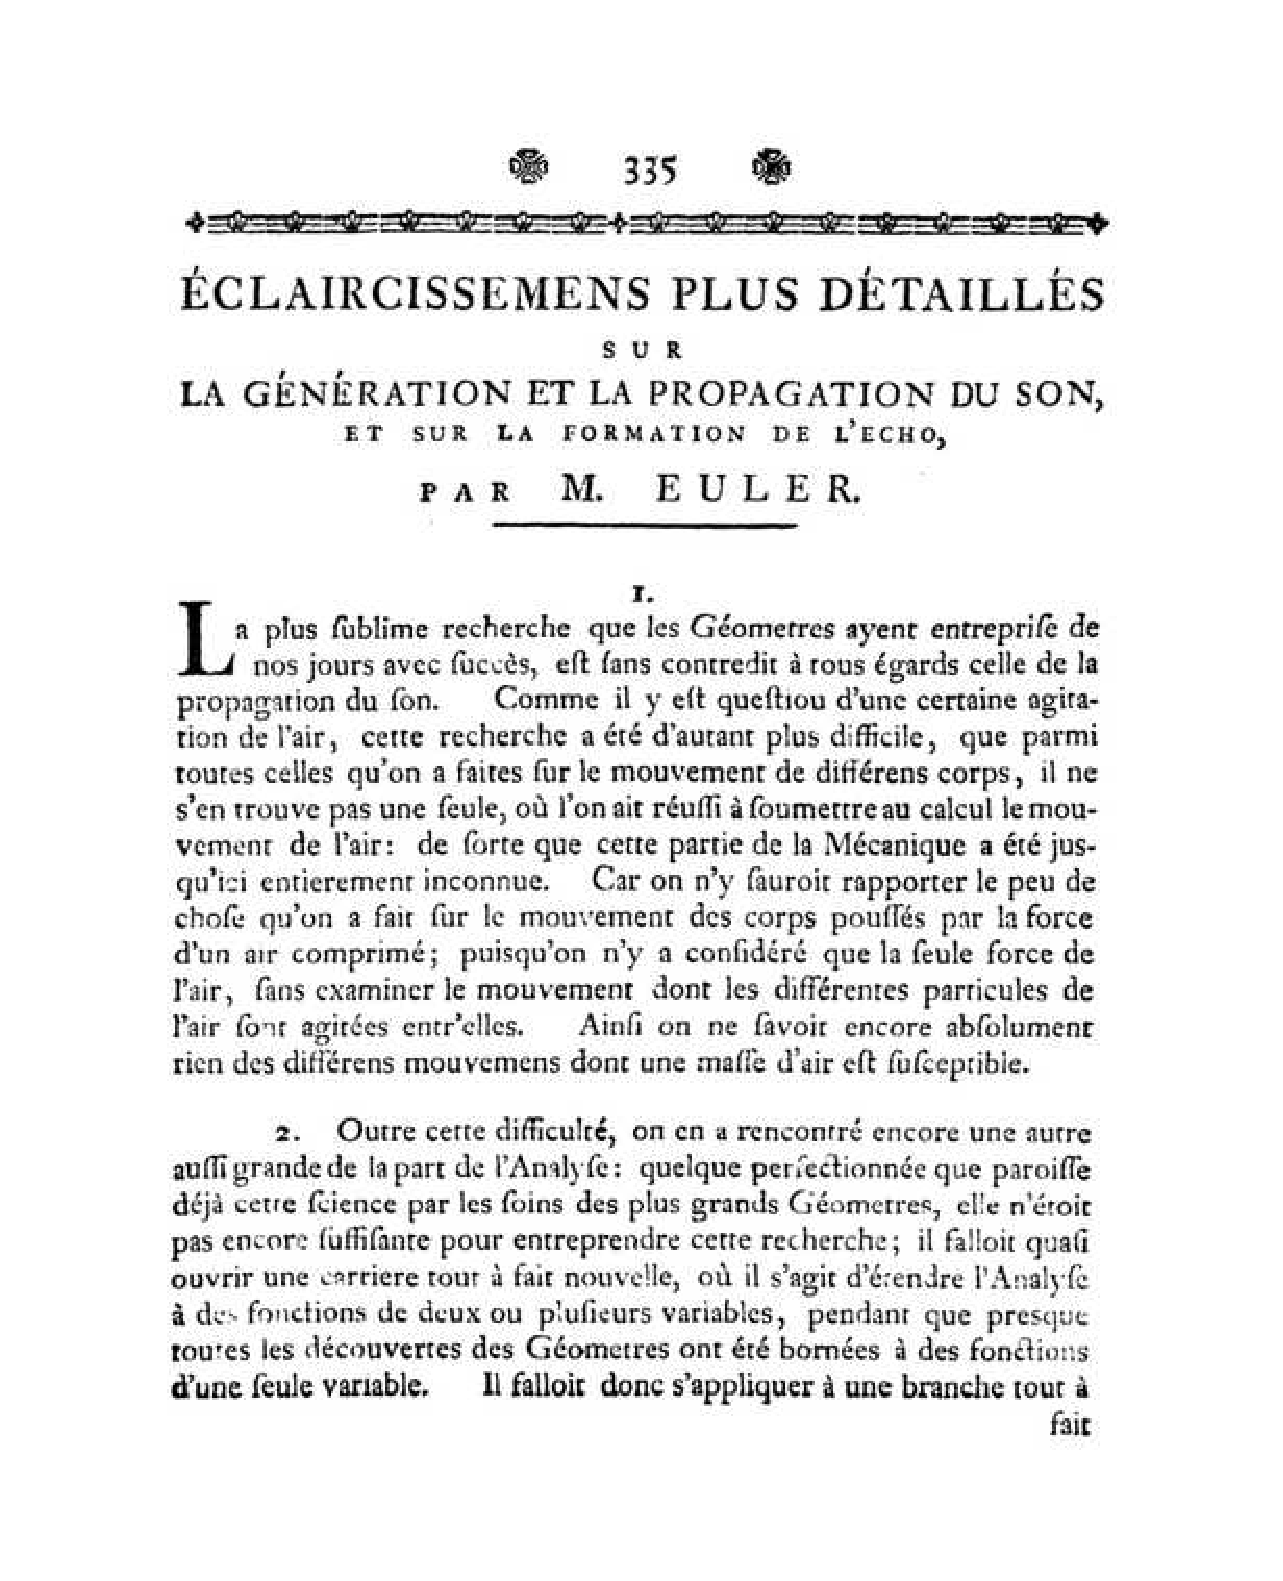
\includegraphics[trim=0.0cm 2.0cm 0.0cm 2.0cm,clip,scale=0.63]{Euler/Euler_p1_1765.eps}

\hspace{-1.3cm}
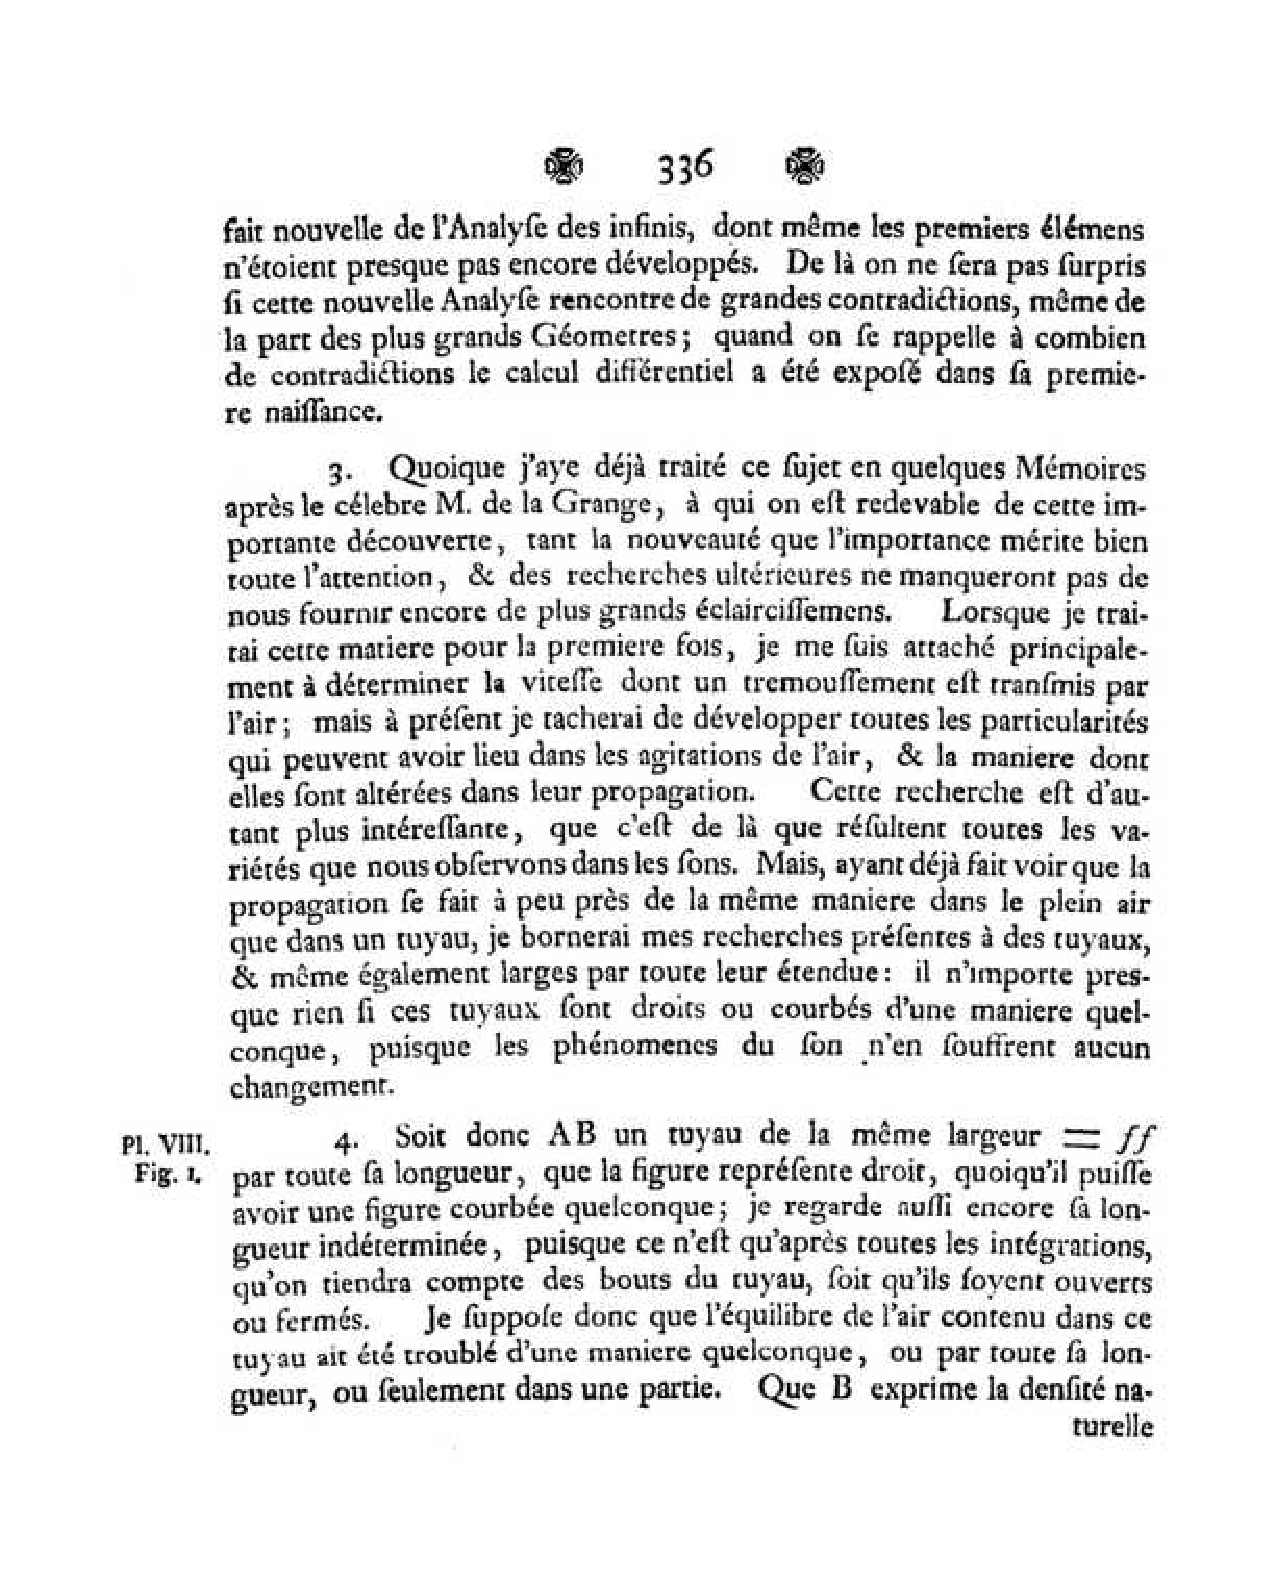
\includegraphics[trim=0.0cm 7.6cm 0.0cm 2.0cm,clip,scale=0.63,angle=-0.5]{Euler/Euler_p2_1765.eps}
\end{figure}

\begin{figure}[!h]
\centering
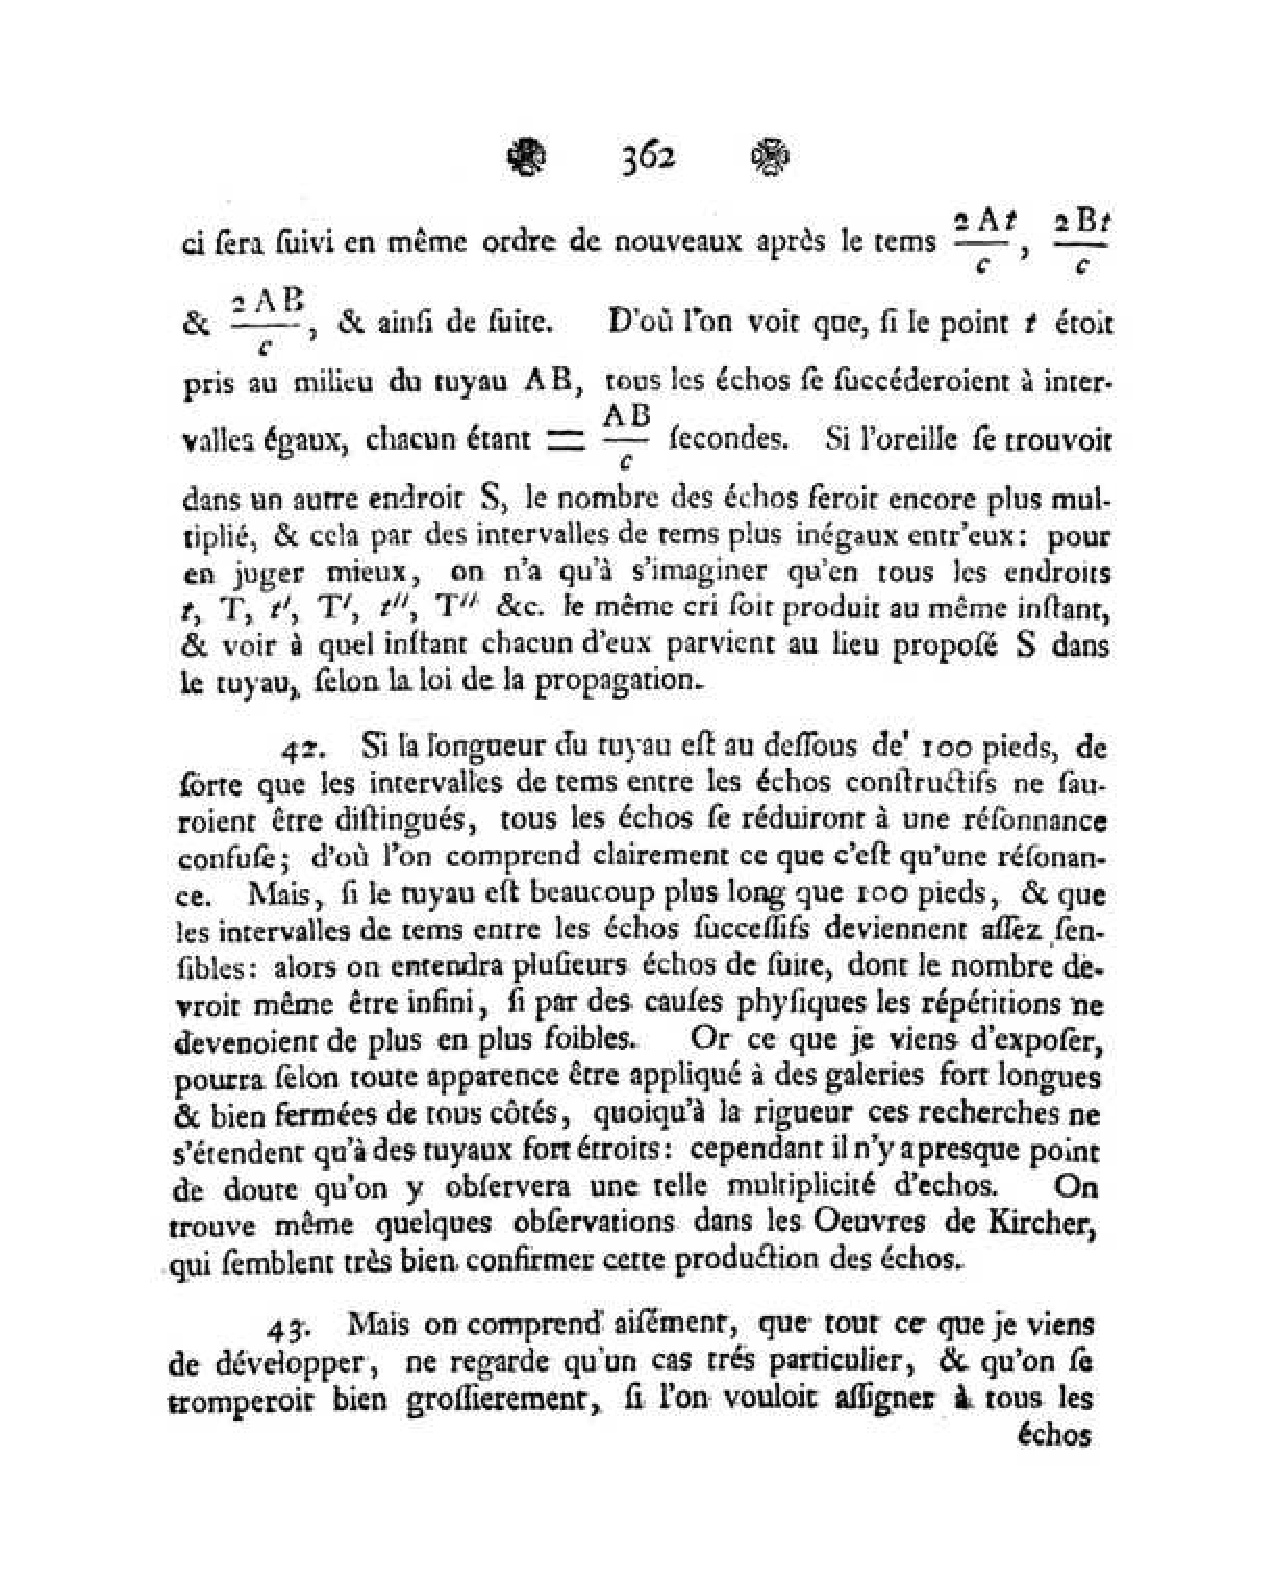
\includegraphics[trim=0.0cm 1.5cm 0.0cm 21.45cm,clip,scale=0.63]{Euler/Euler_p28_1765.eps}

\hspace{-0.5cm}
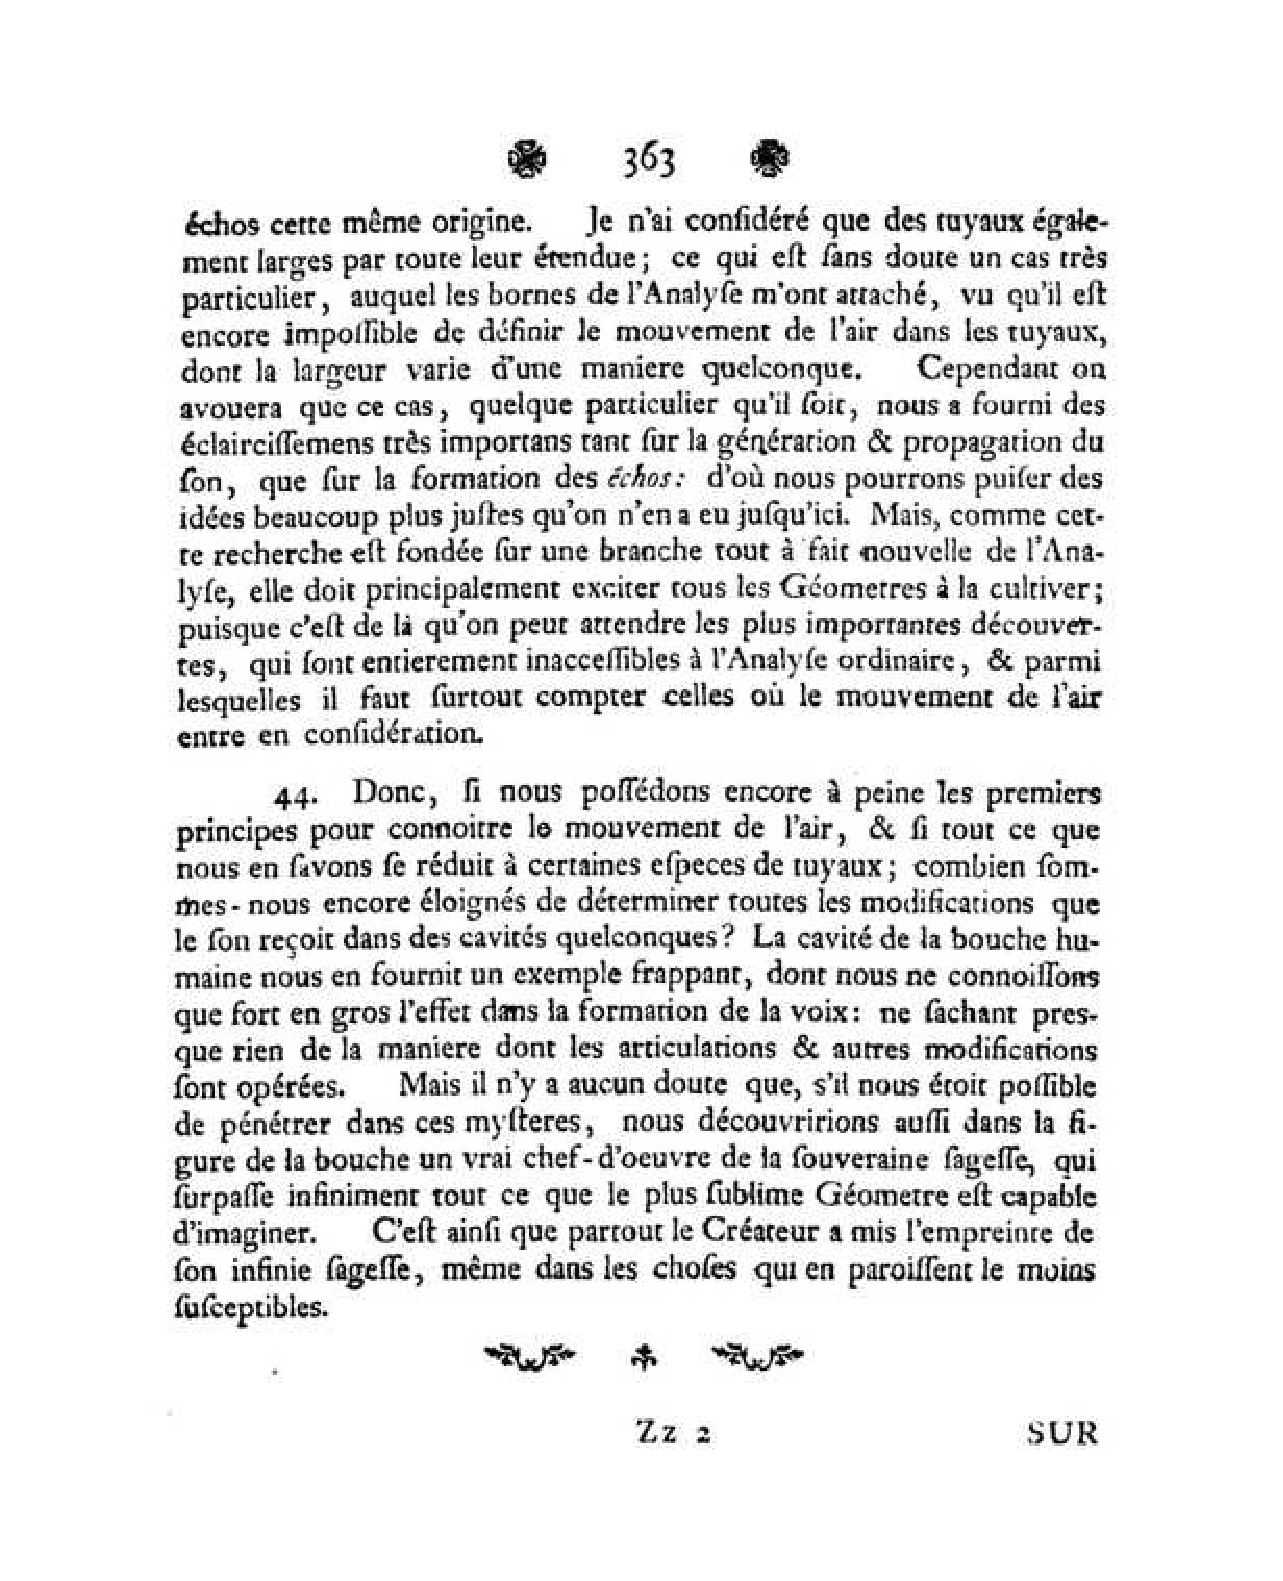
\includegraphics[trim=0.0cm 1.0cm 0.0cm 2.0cm,clip,scale=0.63,angle=0.2]{Euler/Euler_p30_1765.eps}
\caption*{The beginning and ending of the last of Euler's \citeyearpar{Euler_1767} many studies that he contributed on sound propagation. He had derived the basic equations of fluid mechanics a decade earlier \citeyearpar{Euler_1757}. The almost 20 year long controversy in which he opposed d'Alembert on the existence of discontinuous solutions to the wave equation was solved, paving the way to the concept of a wave.
In the meanwhile, the repeated canon shot experiences had sown doubts on Newton's isothermal estimate of the speed of sound, and \citet{Lagrange_1761} solved the wave propagation problem with his adjoint approach.}
\label{fig:Euler_conclusion}
\end{figure}

%``\textit{La plus sublime recherche que les Géomètres aient entreprise de nos jours avec succès, est sans contredit à tous égards celle de la propagation du son. Comme il y est question d'une certaine agitation de l'air, cette recherche a été d'autant plus difficile, que parmi toutes celles qu'on a faites sur le mouvement des différents corps, il ne s'en trouve pas une seule, où l'on ait réussi à soumettre au calcul le mouvement de l’air ; de sorte que cette partie de la Mécanique a été jusqu'ici entièrement inconnue. [...] Ainsi on ne savait encore absolument rien des différents mouvements dont une masse d’air est susceptible.}''

%'''
\clearpage
\thispagestyle{empty}
\skippage %saut de page si nécessaire
%'''

\part{Un titre imposant}
\label{part2:}


%'''
\clearpage
\thispagestyle{empty}
\skippage %saut de page si nécessaire
%'''

\chapter{J'ai quelque chose à vous dire}
\label{part2:chap1:monPremierChapitre}


%%%%%%%%%%%%%%%%%%%%%%%%%%%%%%%%%%%%%%%
%%%%%%%%%%%%%%%%%%%%%%%%%%%%%%%%%%%%%%%
\section{Introductory discussion}
%%%%%%%%%%%%%%%%%%%%%%%%%%%%%%%%%%%%%%%
%%%%%%%%%%%%%%%%%%%%%%%%%%%%%%%%%%%%%%%

"Avant donc que d'écrire, apprenez à penser.
Selon que notre idée est plus ou moins obscure, l'expression la suit, ou moins nette, ou plus pure.
Ce que l'on conçoit bien s'énonce clairement. Et les mots pour le dire arrivent aisément"

\begin{flushright}
Nicolas Boileau, \textit{L'art poétique}, 1674.
\end{flushright}




\addcontentsline{toc}{part}{Conclusion}
\part*{Conclusion}
\label{part3:}
\markboth{Conclusion}{}
"Alles hat ein Ende nur die Wurst hat zwei."

\begin{flushright}
Stephan Remmler, 1986.
\end{flushright}


%'''
\clearpage
\thispagestyle{empty}
\skippage %saut de page si nécessaire
%'''



\clearpage

\bibliographystyle{apalike}
% \bibliographystyle{plain}  
%\renewcommand*{\contentsname}{B\MakeLowercase{ibliography}}
%\renewcommand*{\refname}{REFERENCES}
 

%================================================================
% https://tex.stackexchange.com/questions/78550/how-to-modify-the-headers-of-this-book-to-lower-case
\renewcommand{\chaptermark}[1]{\markboth{#1}{}}
\renewcommand{\sectionmark}[1]{\markright{#1}}
\pagestyle{fancy}
\fancyhf{}
%\fancyhead[LE,RO]{\thepage}
%\fancyhead[LO]{\itshape\nouppercase{\rightmark}}
%\fancyhead[RE]{\itshape\nouppercase{\leftmark}}
%\renewcommand{\headrulewidth}{0pt}
%================================================================
%\fancyhead[R]{\ifthenelse{\isodd{\value{page}}}{References}{}} % from the preambule of this script
\fancyhead[L]{\ifthenelse{\isodd{\value{page}}}{}{References}}
\fancyfoot[R]{\ifthenelse{\isodd{\value{page}}}{\thepage}{}}
\fancyfoot[L]{\ifthenelse{\isodd{\value{page}}}{}{\thepage}}


\bibliography{biblio}

\clearpage

\thispagestyle{empty}
\vspace{-10cm}

%%% Rajouter ici l'autorisation de soutenance
% \includegraphics[trim=2.5cm 3.0cm 2.5cm 2.0cm,clip,width=0.95\textwidth,clip]{appendix/Autosout.eps}


\end{document}
